\documentclass[5p,times,numbers,authoryear]{elsarticle}

\usepackage{ctex}
\usepackage{lineno}%,hyperref}
\usepackage[colorlinks,citecolor=blue]{hyperref}

\usepackage{graphics}
\usepackage{graphicx}
\usepackage{subfigure}
\usepackage{enumitem}
\usepackage{helvet}
\usepackage{courier}
\usepackage{diagbox}
\usepackage{amsmath}
\usepackage{multirow}
\usepackage{booktabs}
\usepackage{makecell}
\usepackage{amssymb}
\usepackage{threeparttable}
\usepackage[justification=centering]{caption}
\usepackage[linesnumbered,ruled,vlined,commentsnumbered]{algorithm2e}
\usepackage{color}
\usepackage{xcolor}
\usepackage{colortbl}
\usepackage{float}
\usepackage{bm}
\usepackage[normalem]{ulem} % use normalem to protect \emph
\newcommand\hl{\bgroup\markoverwith
  {\textcolor{yellow}{\rule[-.5ex]{2pt}{2.5ex}}}\ULon}

\usepackage{hyperref}
\usepackage{breakurl}

\newtheorem{definition}{Definition}
\def\boxend{\hspace*{\fill} $\Box$}
\newcommand{\comment}[1]{}
\renewcommand{\multirowsetup}{\centering}

\journal{Computers in Human Behavior}

\usepackage{appendix}

\begin{document}

\begin{frontmatter}

\title{Stress-Buffering Pattern of Positive Events on Adolescents: \\
An Exploratory Study based on Social Networks}


\begin{abstract}
Stress was viewed as the leading cause of public mental health issues. Positive events, however, could act as a buffer against stress. Since stress-buffering effects of positive events in previous studies were mainly examined by subjective self-reporting, continuous tracking research at individual behavioral levels still remains to be explored. In this study, we collected microblogs (n=27,346) from a group of high school students  (n=500) to examine the relationship between positive events and stress-buffering patterns at both content and behavioral levels. Through a pilot study of scheduled exam intervals under the two situations:
1) existing neighboring scheduled positive events (n=75) and 2) no neighboring positive events,
we found that students during exams with neighboring positive events appeared exhibited less stress intensity and more stable stress fluctuations.
Most students talked less about exams when positive events happened nearby, with lower frequency and lower ratio.
Hypothetical tests for stress-buffering effects of positive events and monotonous changes of stress intensity under the impact of positive events were further conducted based on automatically extracted positive events (n=1,914) from microblogs.
Results showed stress-buffering effects of positive events were closely correlated with adolescents�� stress change modes, microblog linguistic expressions, and posting behaviors.
The occurrence of positive events was verified to offset the impact of stressor events through talking about positive topics at the same time.
Adolescents tended to post more forwarded microblogs, more positive microblogs and less stressful microblogs when positive events appeared,
while the total frequency of microblogs didn't appear obvious change under the impact of positive events.
The study also showed that positive events buffered monotonous changes of stress intensity caused by stressor events.
Based on these theoretical findings, stress-buffering patterns of positive events were further incorporated into the problem of adolescent stress prediction and improved predictive performance.
This study could inform the use of social network to reach and track the mental status transition of adolescents under stress. The theoretical and practical implications, limitations of this study and future work were discussed.
\end{abstract}

\begin{keyword}
stress-buffering, positive events, microblogs, adolescents
\end{keyword}
\end{frontmatter}

\section{Introduction}
\emph{Motivation}: Life is always full of ups and downs.
Accumulated stress could drain inner resources,
leading to psychological maladjustment, depression and even suicidal behaviours \citep{Nock2008Suicide}.
Compared with adults, young people exhibit more exposure to stress
due to the immature inner status and lack of experience \citep{older}.
According to the latest report released by American Psychological Association in 2018,
91\% of youngest adults had experienced physical or emotional symptoms due to stress in the past month compared to 74\% of adults \citep{APA2018}.
More than 30 million Chinese adolescents are suffering from psychological stress,
and nearly 30\% of them have a risk of depression \citep{ChinaTeen2019}.
Stress-induced mental health problems are becoming an important social issue worldwide.

On the other hand, positive life events, such as satisfying social interactions,
excellent academic performance and pleasant entertainment activities,
could exert protective effects on emotional distress in both directly and indirectly ways by \emph{'buffering'} ~\citep{Shahar2002Positive, Cohen2010Positive},
with respect to physiological, psychological, and social coping resources~\citep{Cohen1984Positive,Needles1990Positive}.
Researchers indicated that positive events mitigated the relation between negative events and maladjustment in samples of adolescents experiencing family transitions \citep{Doyle2003Positive}.
The written expression of positive feelings had also been proven to prompt increased cognitive re-organization among an undergraduate student group \citep{Coolidge2009A}.
Positive events also have been linked to medical benefits, such as improving mood, serum cortisol levels, and lower levels of inflammation and hypercoagulability \citep{Caputo1998Influence,Jain2010Effects}.
Thus, tracking the state of stress-buffering is important for understanding the mental status of stressed individuals.
%------------

\emph{Existing solutions}:
Previous studies have been focusing on conducting measurement of positive events and stress-buffering state after events through questionnaires,
including Hassles \& Uplifts Scales~~\citep{Kanner1981Comparison},
Perceived Benefit Scales~~~~~\citep{Mcmillen1998The},
Interpretation of Positive Events Scale~\citep{Alden2008Social}
and Adolescent Self-Rating Life Events Checklist~~~\citep{Jun2008Influence}.
Recent scholars have demonstrated the feasibility to sense and predict users' stress from social networks~\citep{XueUbicomp13,Xue2014Detecting,Lin2014User,Li2015When,Li2015Predicting,Li2015Using,
Li2017Analyzing,Li2017Exploring}
through content (linguistic text, emoticons, pictures)
and behavioral (abnormal posting time, comment/response actions) measures.

If we view the aforementioned traditional studies on positive events as static sensing of stress-buffering,
this study approaches the problem to the dynamic process of stress-buffering
and aims at a solution at both microblogging content and behavioral levels under the hypothesis
that the occurrence of positive events can be reflected in adolescents' microblogs.
Since the subjective self-report investigations are susceptible to many factors,
such as social appreciation and pressures from measurement scenarios,
microblogging characteristics at the behavioral level are objective expressions that can assist content characteristics.

Another difference from the previous studies lies in that,
despite the unique advantages of social networks over traditional survey methods in offering self-expressed content and behavioral information,
previous microblog-based researches stopped at the analysis of stress,
and none went further to capture positive events that may play a key role in adolescents' stress coping mechanism.
For example, it is ��hiking tomorrow�� that might simultaneously occur and be expressed in microblogs with ��losing the exam today��.
If we couldn't know anything about positive events,
is the stress unilaterally detected is the real stressful state of the current youth?
Understanding stress-buffering patterns of positive events
is helpful in precisely predicting and guiding stressful adolescents coping with stress.

\emph{Our work}:
To this end,
this paper proposes to study adolescent stress in a dual perspective of stress generation and stress-buffering,
and view it as the superposition effect of stressors and positive events.
By investigating the connection between positive events and stress changes
reflected through adolescents' microblogging content and behaviors,
we discover stress-buffering patterns of positive events and further predict future stress under such mitigation.
Exploiting stress-buffering effects of positive events
is also advantageous in handling the confusing situation
whether an adolescent who doesn't express stressful information from microblogs is actually under stress.

However, capturing the stress-buffering process of positive events is not a trivial task.
Three fundamental challenges need to be addressed:
1) What are the criteria to depict stress-buffering?
2) What is the latent connection between positive events and adolescents' stress-buffering reflections from microblogs?
3) How to extract positive events and its impact interval from microblogs?

%1
A pilot study was firstly conducted on the microblog data (n=27,346) of a group of high school students (n=500)
associated with the school's scheduled positive events (n=75) and stressor events (n=122).
Stressful intervals were divided into two comparative categories:
intervals impacted by scheduled positive events (denoted as U-SI, n=259)
and intervals not impacted by scheduled positive events (denoted as SI, n=518).
After observing the posting behaviors and contents of stressed students in both SI and U-SI groups,
several implications were discussed to guide the next step study.

%3
Motivated by the implications from the pilot study,
we modeled the connection between positive events and adolescents' stress-buffering reflections
as the statistical difference in two comparative situations SI and U-SI.
Three groups of measures were adopted to depict adolescent stress-buffering at period-level:
stress change modes, linguistic expressions and posting behaviours.
Positive events buffered monotonous changes of stress intensity
Monotonous changes of stress intensity buffered by positive events were measured in temporal order.
%4
As an exploration,
according to the occurrence of automatically extracted positive events,
we covered its stress-buffering effects into each time unit
and integrated such effect into stress prediction.

%2
In this paper,
to realize automatically extraction of positive events,
we stood upon and extended previous stress and event detection works.
A Chinese linguistic parser model was applied to extract positive events in the linguistic structure
\emph{[type, (act, doer, description)]}.
We followed the categorization of adolescents' positive events in six dimensions (entertainment, school life, romantic, pear relationship, self-cognition, family life) and extended SC-LIWC lexicons to 2,606 phases.
Stressful intervals (SI) and stressful intervals impacted by positive events(U-SI) were identified according to temporal orders.

The rest of the paper is organized as follows.
We review the literature in section \ref{sec:related},
and introduce the pilot study in section \ref{sec:obs}.
The procedure for extracting positive events is presented in section \ref{sec:frame1}.
The connection between positive events and adolescents' stress-buffering from microblogs are discussed and modeled in section \ref{sec:frame2}.
We present the experimental results in section \ref{subsec:experiment},
and extend the study to integrating stress-buffering patterns into future stress prediction in section \ref{subsec:predict}.
Future work is discussed in section \ref{sec:conclude}.

\section{Literature Review}
\label{sec:related}
\subsection{Stress-buffering Function of Positive Events}
Positive events have been verified as protective factors against daily stress~\citep{Ong2006Psychological,Bono2013Building}, loneliness~\citep{Chang2015Loneliness}, suicide~\citep{Evan2014Social} and depression~\citep{Santos2013The}.
Through exploring naturally occurring daily stressors, \citep{Ong2006Psychological} found that over time,
the experience of positive emotions functions to assist high-resilient individuals to recover effectively from daily stress.
Through a three-week longitudinal study, \citep{Bono2013Building} examined the correlation between employee stress and health and positive life events, and concluded that naturally occurring positive events are correlated with decreased stress and improved health.
\citep{Chang2015Loneliness} investigated the protective effect of positive events in a sample of 327 adults, and found that the positive association between loneliness and psychological maladjustment was found to be weaker for those who experienced a high number of positive life events, as opposed to those who experienced a low number of positive life events.
This is assistant with the conclusion made by \citep{Evan2014Social} that positive events acted as protective factors against suicide individually and synergistically when they co-occurred,
by buffering the link between important individual differences risk variables and maladjustment.
In the survey made by \citep{Santos2013The},
strategies of positive psychology were also checked as potentially tools for the prophylaxis and treatment of depression, helping to reduce symptoms and for prevention of relapses.

The protective effect of positive events was hypothesized to operate in both directly (i.e., the more positive events people experienced, the less stress they perceived)
and indirectly ways by \emph{'buffering'} the effect of stressors ~\citep{Cohen2010Positive,Shahar2002Positive},
with respect to physiological, psychological, and social coping resources ~\citep{Cohen1984Positive, Needles1990Positive}.
\citep{Folkman2010Stress} identified three classes of coping mechanisms that were associated with positive emotion during chronic stress: positive reappraisal, problem-focused coping, and the creation of positive events.
Due to the immature inner status and lack of experience,
adolescents exhibit more sensitive to stressors
(i.e., exams, heavy homework, isolated by classmates, family transitions),
living with frequent, long-term stress~\citep{older}.
In this situation,
positive events could help reinforce adolescents' sense of well-being~\citep{Coolidge2009A},
restore the capacity for dealing with stress~\citep{Doyle2003Positive},
and also have been linked to medical benefits, such as improving mood, serum cortisol levels, and lower levels of inflammation and hyper coagulability \citep{Jain2010Effects,Caputo1998Influence}.
The present study will be based on the consensus conclusions from the above studies.

To assess the stress-buffering effect of positive events,
scholars conducted many studies based on self-support methods.
For example,
\citep{Kanner1981Comparison} conducted Hassles \& Uplifts Scales,
and concluded that the assessment of daily hassles and uplifts might be a better approach to the prediction of adaptational outcomes than the usual life events approach.
To measure negative interpretations of positive social events,
\citep{Alden2008Social} proposed the Interpretation of Positive Events Scale, and analyzed the relationship between social interaction anxiety and the tendency to interpret positive social events in a threat-maintaining manner.
\citep{Mcmillen1998The} proposed the Perceived Benefit Scales as the new measures of self-reported positive life changes after traumatic stressors, including lifestyle changes, material gain, increases in self efficacy, family closeness, community closeness, faith in people, compassion, and spirituality.
Specific for college students,
\citep{Jun2008Influence} investigated in 282 college students using the Adolescent Self-Rating Life Events Checklist, and found that the training of positive coping style was of great benefit to improve the mental health of students.
The above explorations based on self-report investigations
were difficult to exclude interference from external factors (i.e., social appreciation, pressure from measurement scenarios).
Meanwhile, due to the lack of manpower and effective scientific methods,
most scholars relied on a limited number of measurements,
thus continuous measurements of stress-buffering process were difficult to carry out.

\subsection{Measures and Stress Analysis from Social Networks}
As billions of adolescents are recording their life through social networks (e.g., micro-blog, Twitter, Facebook),
researchers explored to apply psychological theories into social network based data mining techniques,
thus to better understand user' psychological status from the self-expressed public data source.
Multiple content and user behavioral measures have been proven effective in user mental health analysis,
including time series curve analysis of stress~\citep{Li2015When,Li2015Using}, topic words~\citep{XueUbicomp13}, abnormal posting time~\citep{Xue2014Detecting},
online shopping behaviors~\citep{DBLP:conf/apweb/Zhao0XLF16},
human mobility features~\citep{DBLP:conf/dasfaa/JinXLF16}, comment/response actions~\citep{Liang2015Teenagers}
and high dimensional multimedia features~\citep{Lin2014User}.
For example,
\citep{XueUbicomp13, Xue2014Detecting} proposed to detect adolescent stress from single post utilizing machine learning methods by extracting stressful topic words, abnormal posting time, and interactions with friends.
\citep{Lin2014User} constructed a deep neural network to combine the high-dimensional picture semantic information into stress detecting.
Based on the stress detecting result,
\citep{Li2015Predicting}\cite{Li2015Using}\cite{Li2015When} adopted a series of multi-variant time series prediction techniques (i.e., Candlestick Charts, fuzzy Candlestick line, Seasonal Autoregressive Integrated Moving Average model) to predict future stress trend.
Taking the linguistic information into consideration,
\citep{Li2017Exploring} employed a Nonlinear autoregressive with External Input Neural Network to predict a teen's future stress level referred to the impact of co-experiencing stressor events of similar companions.
\citep{Li2017Analyzing} proposed to detect stressor events from microblog content
and analyze stressful intervals based on posting rate.
All above studies focused on the discussion of stress detection on social networks.
This paper starts from a completely new perspective,
and focuses on the stress-buffering effect of positive events in adolescents' stress coping process.
Thus we push forward the study from how to find stress to the next more meaningful stage: how to cope with stress.

\subsection{Correlation Analysis Models for Multivariate Time Series}
Basic correlation analysis models on time series focused on univariate data have been well studied.
As the most widely adopted model,
the Pearson correlation analysis \cite{Cohen1988Statistical} measures the linear correlation between two variables $X$ and $Y$.
One inevitable defect of Pearson correlation is its sensitivity to outlier values.
To overcome such drawback,
Spearman Rank correlation \cite{C1987The}
and Kendall Rank correlation \cite{Mcleod2011Kendall}
were proposed based on Pearson correlation.
While Pearson correlation estimates linear relationships,
Spearman correlation estimates monotonic relationships (whether linear or not),
and are calculated as the Pearson correlation between the rank values of two variables.
The Kendall Rank correlation mainly assesses the similarity of the orderings of the data when ranked by each of the quantities.
The above correlation models are usually used to estimate relationship between single-dimensional variables,
and cannot be adopted directly in social network based scenario.

For multivariate time series analysis,
two-sample based models were widely adopted.
Such kind of models were deduced to check whether two samples come from the same underlying distribution,
which was assumed to be statistically unknown.
Correspondingly,
various kernel \citep{Sch2006A} and distance-based models \citep{Schilling1986Multivariate} were proposed.
\citep{Sch2006A} proposed to transform the distance between two variables and nearest neighbors into a reproducing kernel hilbert pace, and solve the problem using Maximum Mean Discrepancy.
\citep{Schilling1986Multivariate} adopted the $r$-nearest neighbor based model to partition two set of event driven time series data.
The global proportion of the right divided neighbors were calculated to estimate whether there existed statistically difference between the two sets.
This paper adopted the $r$-nearest neighbor based two-sample model in our problem,
thus to measure the distance and correlation between two multi-dimension variables depict
the stress-buffering patterns of positive events.

\section{Data Observation: A Pilot Study on the Stress-buffering Effect of School Scheduled Positive Events}
\label{sec:obs}
\paragraph{Microblogs} Microblogs of students coming from Taicang High School were collected from January 1st, 2014 to September 1st, 2017.
We filtered out 121 active students according to their posting frequency from over 500 students,
and collected their microblogs throughout the whole high school career.
Totally 27,346 microblogs were collected in this research,
where 226 microblogs per student on average, 1,421 microblogs maximally and 102 posts minimally.
To protect the privacy, all usernames were anonymized during the experiment.

\paragraph{Scheduled events} The list of weekly scheduled school events,
with detailed description involved in the event (grade, exact start and end time),
were collected from the school's official website\footnote{http://stg.tcedu.com.cn/col/col82722/index.html} from February 1st, 2014 to August 1st 2017.
There were 126 stressor events and 75 positive events in total.
Examples of scheduled positive and stressor events in high school life are listed shown in Table~\ref{tab:example}.
There were 2-3 stressor events and 1-2 positive event scheduled per month in current study.
Figure~\ref{fig:example} shows three examples of a student's stress fluctuation during three mid-term exams,
where the positive event \emph{campus art festival} was scheduled ahead of the first exam (\emph{example a}),
the positive event \emph{holiday} happened after the second exam (\emph{example b}),
and no scheduled positive event was found nearby the third exam (\emph{example c}).


\begin{table}[H]
\caption{\small{Examples of school scheduled positive and stressor events.}}
\label{tab:example}
\resizebox{.45\textwidth}{9mm}{
\small{
\begin{tabular}{cccc}
\toprule
Type & Date	& Content	& Grade	\\
\midrule
stressor event & 2017/4/16 & first day of mid-term exam & grade1,2\\
positive event & 2016/11/5 & campus art festival & grade1,2,3\\
\bottomrule
\end{tabular}
}
}
\end{table}

\begin{table}[h]
\centering
\caption{\small{Examples of academic related keywords.}}
\label{tab:studyWords}
\small{
\begin{tabular}{c}
\toprule
exam, fail, review, score, test paper, rank, pass, math, chemistry\\
homework, regress, fall behind, tension, stressed out, physics,\\
nervous, mistake, question, puzzle, difficult, lesson, careless\\
\bottomrule
\end{tabular}
}
\end{table}


\begin{figure}[H]
\centering
\includegraphics[width=\linewidth]{figs/exampleWave.eps}
\caption{\small{Examples of school scheduled positive events, stressor events, and a student's stress fluctuation}}
\label{fig:example}
\end{figure}

To further observe the effect of positive events on stressed students,
we collected all stressful intervals surround the scheduled exams over the 121 students during their high school career
applying the interval detection method in ~\citep{Li2017Analyzing}.
For each student, we divided all stressful intervals into two sets:
1) In the original sets, stress was caused by a stressor event, lasting for a period,
and no other intervention (namely, positive event) occured.
We called the set of such stressful intervals as \textbf{SI};
2) In the other comparative sets,
the stressful interval was impacted by a positive event,
we called the set of such stressful intervals as \textbf{U-SI}.
Thus the difference under the two situations (sets) could be seen as the stress-buffering effect
conducted by the positive event.
We identified 518 exam related stressful intervals (SI)
and 259 stressful intervals impacted by four typical scheduled positive events (U-SI)
('practical activity', 'new year party', 'holiday', 'sports meeting') from the students' microblogs.
Six measures in the above two conditions were considered:
the \emph{accumulated value of stress}, the \emph{average value of stress} (per day),  the \emph{maximal value of stress} (per day),
the \emph{RMS value of stress},
the \emph{frequency of academic topic words}, and the \emph{ratio of academic stress among all types of stress}.
Since our target was to track the impact of positive events for students under stress,
based on previous research~\cite{XueUbicomp13},
we detected the stress level (ranging from 0 to 5) for each post.
For each student,
the stress value per day was aggregated by calculating the average stress of all posts.
Examples of academic related keywords were listed in table \ref{tab:studyWords}.
The average value of each measure over all eligible slides was calculated.


\begin{figure}[h]
\centering
\includegraphics[width=\linewidth]{figs/barUSI.eps}
\caption{\small{Comparing stress (average value of all students) during exam intervals in two situations:
1) intervals affected by neighboring positive events (U-SI), 2) no positive events occurred nearby (SI).}}
\label{fig:frequencyBar}
\end{figure}

\begin{figure}[h]
\centering
\includegraphics[width=\linewidth]{figs/activity.eps}
\caption{\small{Comparing students' stress fluctuations during exam intervals in U-SI and SI sets.}}
\label{fig:frequency}
\end{figure}

\paragraph{Results}
As shown in figure~\ref{fig:frequencyBar},
comparing each measure of scheduled exam intervals under the two situations:
1) existing neighbouring positive events (U-SI) and 2) no neighbouring scheduled positive events (SI),
we found that students during exams with neighbouring positive events appeared exhibited less stress intensity
(78.13\% reduction in average stress, 95.58\%  reduction in cumulative stress, 57.20\%  reduction in maximal stress)
and more stable stress fluctuations (47.93\% reduction in RMS values of stress).
Further, the frequency of academic topic words (table \ref{tab:studyWords} for examples)
and the ratio of academic stress in each interval were calculated.
Most students talked less about exams when positive events happened nearby,
with lower frequency (84.65\% reduction) and lower ratio (89.53\% reduction).
The statistic result shows clues about the impact of scheduled positive events,
which is constant with the psychological theory ~\citep{Cohen1984Positive, Cohen2010Positive, Needles1990Positive},
indicating the reliability and feasibility of the microblog data set.
However,
this is an observation based on specific scheduled events,
and cannot satisfy the need for automatic, timely, and continuous perception of stress-buffering process.
Therefore, next, we will propose a framework to automatically detect positive events and its impact interval.
Based on this,
the relationship between the impact of automatically extracted positive events
and adolecents' microblogging characteristics will be discussed.


\section{Framework}
\label{sec:frame}
We first introduce the procedure to extract positive event and its intervals from microblogs.
Based on this,
we present a statistical model to depict
the relationship between positive events and adolescents' stress-buffering patterns through three groups of content and behavioral measures.
%Finally, a none-liner time series model was proposed to combine stress-buffering patterns into future stress prediction.
\subsection{Discovery of Positive Events from Microblogs}
\label{sec:frame1}
Let $u$ = $[type,\{doer, act,$ $description\}]$ be a positive event,
where the element \emph{doer} is the subject who performs the \emph{act},
and \emph{descriptions} are the key words related to $u$.
According to psychological scales ~\citep{Jun2008Influence,hassles},
adolescent positive events mainly focus on six dimensions,
as $\mathbb{U} =\{$ 'entertainment', 'school life', 'romantic', 'pear relationship', 'self-cognition', 'family life'$\}$. We constructed our lexicon for six-dimensional positive events from two sources.
The basic positive words are selected from the psychological lexicon C-LIWC (expectation, joy, love, surprise)~\citep{Tausczik2010The}.
Then we built six topic lexicons by expanding basic positive words from adolescent microblogs,
containing 452 phrases in 'entertainment',
273 phrases in 'school life',
138 phrases in 'romantic',
91 phrases in 'peer relationship',
299 phrases in 'self-recognition' and 184 phrases in 'family life', with totally 2,606 phrases,
as examples shown in table \ref{tab:topicWords}.
Additionally, we labeled \emph{doer} words (i.e., \emph{teacher}, \emph{mother}, \emph{I, we}) in positive lexicons.

\begin{table*}
\centering
\caption{\small{Examples and statistics for topic phrases in six-dimensional lexicons of positive events.}}
\label{tab:topicWords}
\small{
\begin{tabular}{lll}
\toprule
dimension & example words & total \\ \midrule
entertainment  & hike, travel, celebrate, dance, swimming, ticket, shopping, air ticket, theatre, party, Karaoke,& 452\\
                      & self-driving tour, game, idol, concert, movie, show, opera, baseball, running, fitness, exercise & \\
school life    & reward, come on, progress, scholarship,admission, winner, diligent, first place, superior & 273\\
				      & hardworking, full mark,  praise, goal, courage, progress, advance, honor, collective honor& \\
romantic       &  beloved, favor, guard, anniversary,  concern, tender, deep feeling, care, true love, promise, & 138\\
				      & cherish, kiss, embrace, dating, reluctant, honey, sweetheart, swear, love, everlasting, goddess &\\
pear relation  & listener, company, pour out, make friends with, friendship, intimate, partner, team-mate, brotherhood& 91\\
self-cognition & realize, achieve, applause, fight, exceed, faith, confidence, belief, positive, active, purposeful & 299\\
family life    & harmony, filial, reunite, expecting, responsible, longevity, affable, amiability, family, duty & 184\\
\bottomrule
\end{tabular}}
\end{table*}

\begin{table}[h]
\begin{center}
\caption{\small{Examples of automatically extracted positive events from adolescents' microblogs.}}
\small{
\begin{tabular}{|l|} \hline
I am really looking forward to the spring outing on Sunday now. \\
(doer:\emph{I}, act:\emph{looking forward}, description:\emph{spring outing})\\\hline
My holiday is finally coming [smile]. \\
(doer:\emph{My holiday}, act:\emph{coming}, description:\emph{[smile]})\\\hline
First place in my lovely math exam!!! In memory of it.\\
(description:\emph{first place, math, exam, memory})\\\hline
You are always here for me like sunshine. \\
(doer:\emph{You}, description:\emph{sunshine})\\\hline
Thanks all my dear friends hosting the party.
Happiest birthday!!!\\
(doer:\emph{friends}, act:\emph{thanks}, description:\emph{party, birthday})\\\hline
I know my mom is the one who support me forever, no matter \\
when and where. (doer:\emph{mom}, act:\emph{support})\\ \hline
Expecting Tomorrow' Adult Ceremony[Smile][Smile]~~\\
(act: \emph{expecting}, description:\emph{Adult Ceremony})\\\hline
\end{tabular}}
\label{tab:uplifts}
\end{center}
\end{table}

\subsubsection{Linguistic Parser Model}
Positive events were identified through Chinese natural language processing platform \citep{Che2010}.
For each post, after word segmentation, we parsed each sentence to find its linguistic structure,
and then matched the main linguistic components with positive topic lexicons in each dimension.
The linguistic parser model was applied to identify the central verb of current sentence, namely the \emph{act}.
It constructed the relationship between the central verb and corresponding \emph{doer} and \emph{description} elements.
By searching these elements in positive topic lexicons,
the existence of positive events were identified.
Due to the sparsity of posts, the element \emph{act} might be empty.
\emph{Descriptions} were collected by searching all nouns, adjectives and adverbs.
Examples of positive events extracted from adolescents' microblogs are listed in table \ref{tab:uplifts}.
For the post 'Thanks all my dear friends hosting the party. Happiest birthday!!!',
it was processed as \emph{doer='friends', act = 'expecting', description = 'party'},
and \emph{type = 'entertainment'}.

\subsubsection{Impact Intervals of Positive Events}
\label{subsec:interval}
We followed and extended ~\citep{Li2017Analyzing} to identify the impact interval of each positive event to further study its stress-buffering pattern.
The target interval was identified in three steps.

Step1:
Extracted positive events, stressor events and filtered out candidate intervals.
For each candidate interval,
we set its length to more than 3 days and a maximum gap of 1 day between two neighboured stressed days.
Since the stress series detected from microblogs were discrete points,
locally weighted regression ~\citep{Cleveland1988Locally} method was adopted to highlight characteristics of the stress curve.

Step2: Judged stressful intervals through hypothesis testing.
A Poisson based probability model was adopted to measure how confidently the current interval was a stressful interval.
Here the stressful posting rates under stress $\lambda_1$ and normal conditions $\lambda_0$ were modeled as two independent poisson process:
\begin{equation}
Pr[N=n|\lambda_i]=\frac{e^{-\lambda_i T}{(\lambda_i T)}^n}{n!}
\end{equation}
where $i\in\{0,1\}$, $n=0,1,\cdots,\infty$.
We expected that $\lambda_1 > \lambda_0$, and measured the probability as $P(\lambda_1>\lambda_0|N_1, T_1, N_0, T_0)$,
where $N_1, N_0$ are the number of stressful posts, and $T_1, T_0$ are time duration corresponding to $\lambda_1$ and $\lambda_0$.
Without loss of generality, we assume a Jeffreys non-informative prior on $\lambda_1$ and $\lambda_0$,
and inferred the posterior distribution $P(\lambda_1|N_1)$ and $P(\lambda_0|N_0)$ according to Bayes Rule.
Thus for current interval $I_1$ and historical normal interval $I_0$,
the quantified probability $\beta = P(\lambda_1>\lambda_0|I_1,I_0)$ $\in (0,1)$ indicated the confidence
whether $I_1$ was a stressful interval.

Step 3: Divided stressful intervals into SI set and U-SI set.
For a detected stressful interval $I = <t_1,\cdots,t_n>$, we considered the temporal order between $I$ and any detected positive event $u$ happening at time point $t_u$ in three cases:
\begin{itemize}
\item[1)] If the positive event $u$ happened during the stressful interval, i.e., $t_u \in [t_1,t_n]$, the positive interval $I$ was judged as $I \in U-SI$.
\vspace{-0.3cm}
\item[2)] If the positive event happened nearby a stressful interval,
considering the probability that it conducted impact on current stressful interval.
Here the gap between $t_u$ and $I$ is limited to $\xi$, i.e.,
if $t_u \in [t_{1}-\xi, t_1)\cup(t_{n},t_{n}+\xi]$, then $I \in U-SI$.
If a stressful interval satisfies none of the above conditions, we classify it into the SI set.
\vspace{-0.3cm}
\item[3)] Other stressful intervals were divided into U-SI set.
\end{itemize}

\subsection{Hypothesis Test for the Relationship between Positive Events and Adolescents' Stress-buffering}
\label{sec:frame2}
We formulated the relationship between positive events and adolescents' stress-buffering patterns
as a comparison problem between two sets of stressful intervals: the SI set and the U-SI set.
Each interval was modeled as a multi-dimensional vector depicted microblogging characteristics of current adolescent.
Specifically, the multivariate two-sample hypothesis testing method
\cite{Li2017Correlating,Johnson2012Applied} was adopted to model such relationship.
The basic idea was judging whether the multi-dimension points (i.e., stressful intervals)
in set SI and set U-SI were under different statistical distributions.
Assuming the data points in SI and U-SI were randomly sampled from distribution $F$ and $G$, respectively,
then the hypothesis was denoted as:
\begin{equation}
H_0: F = G \quad versus \quad H_1: F \neq G.
\end{equation}
Under such hypothesis,
$H_0$ indicated points in SI and U-SI were under similar distribution,
while $H_1$ meant points in SI and U-SI were under statistically different distributions,
namely positive events conducted obvious stress-buffering effect.

\subsubsection{Statistical Model of Stress-buffering Effect}
\begin{figure*}
\centering
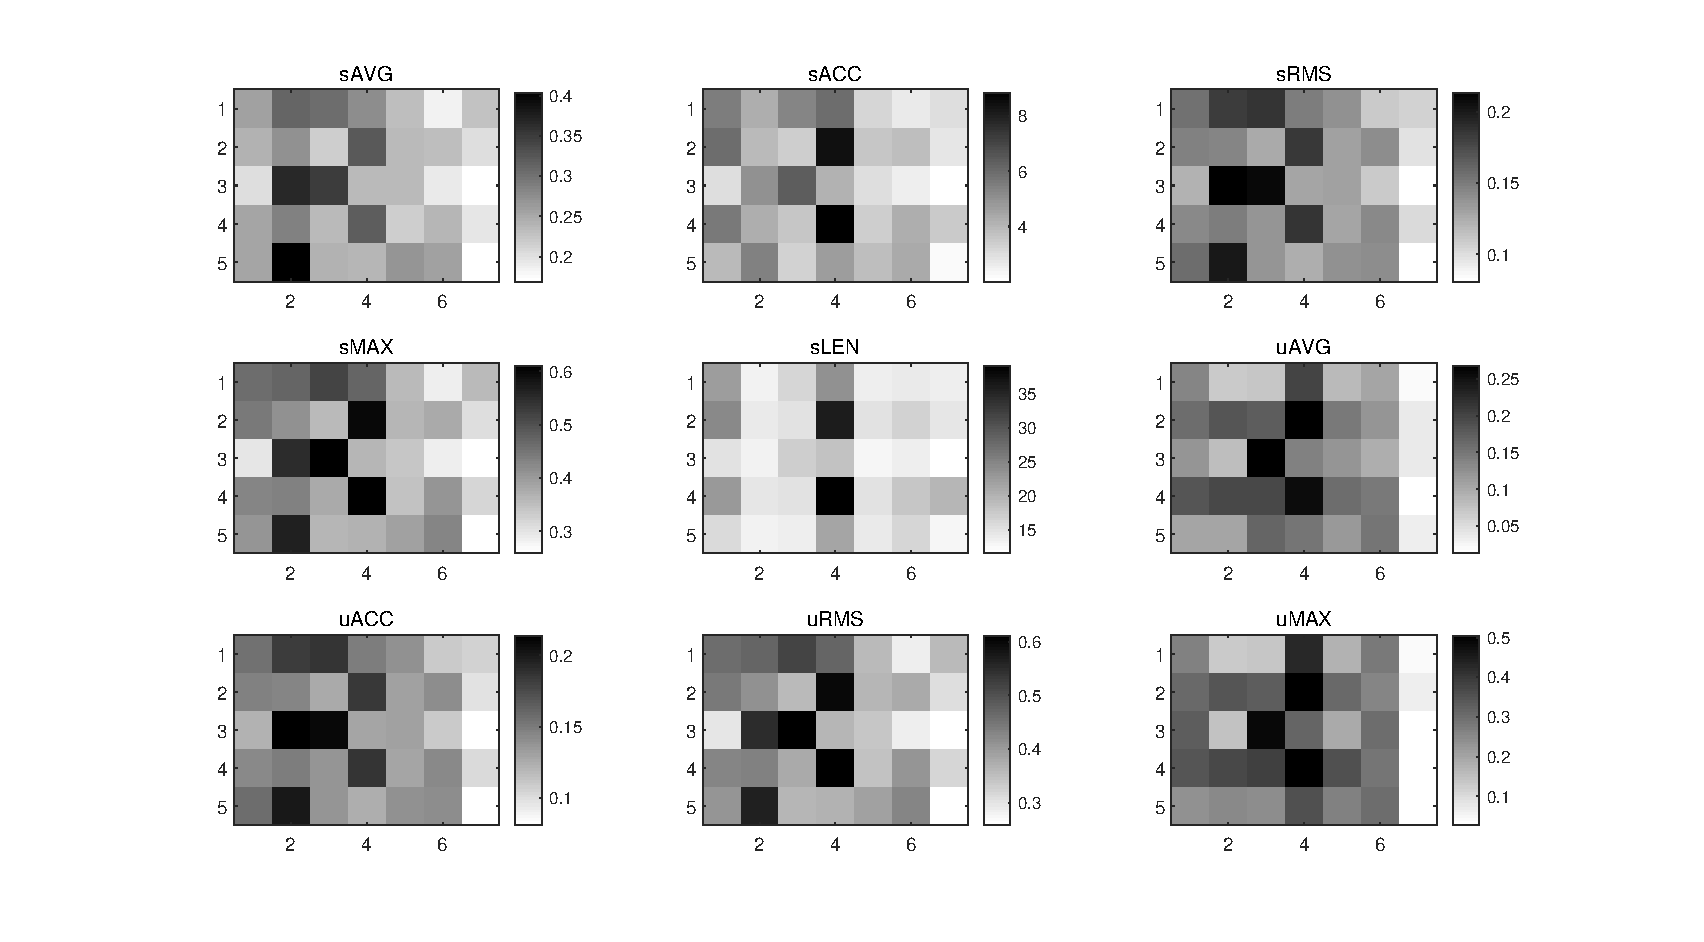
\includegraphics[width=\linewidth]{figs/gray/stress.eps}
\caption{\small{Comparing stress change modes during stressful intervals in two situations:
1) intervals affected by neighboring positive events (U-SI), 2) no positive events occurred nearby (SI).
$P_{1-6}$=\{academic, romantic, peer relationship, self-cognition, family life, entertainment\},
$E_{1-5}$=\{academic, romantic, peer relationship, self-cognition, family life\}.}}
\label{fig:stress}
\end{figure*}
We took the K-Nearest Neighbor based method (\cite{Schilling1986Multivariate}) to judge the existence of significant difference between set SI and set U-SI.
For simplify, we used the symbol $A_1$ to represent set SI,
and $A_2$ represent set U-SI.
For each point $\ell_{x}$ in the two sets,
we expected its top-k similar points belonging to the same set of $\ell_x$.
The Euclidean distance was adopted to calculate the distance of structured points here.
For each point $\ell x \in A=A_1\bigcup A_2$,
let $\textbf{D}^y$ be the feature vector of $\ell_x$,
and $NN_r(\ell_x,A)$ be the function to find the $r-$th nearest neighbor of $\ell_x$.
The $r$-th nearest neighbor of $\ell_x$ was denoted as:
\begin{equation}
\begin{aligned}
& NN_r(\ell_x,A) = \{y | min\{||\textbf{D}^x-\textbf{D}^y ||_2\}, y\in(A/\ell_x)\} &
\end{aligned}
\end{equation}
Let $I_r(\ell_x,A1,A2)$ be the function denoting whether the $r$-th nearest neighbor was in the same set with $\ell_x$:
\begin{equation}
I_r(\ell_x,A_1,A_2) =
\left\{ \begin{array}{ll}
1, \quad if \ell_x \in A_i  \&\& NN_r(\ell_x,A)\in A_i,\\
0, \quad otherwise
\end{array}
\right.
\end{equation}
Let $T_{r,n}$ denote the proportion that pairs containing two points from the same set among all pairs formed by $\ell_x \in A$ and its $k$ nearest neighbors:
\begin{equation}
T_{k,n}= \frac{1}{n\times k}\sum_{i=1}^{n}\sum_{j=1}^{k}I_j(x,A_1,A_2)
\end{equation}
The value of $T_{k,n}$ showed how differently the points in the two testing sets (SI and U-SI) performed.
If the value of $T_{r,n}$ was close to $1$,
it could be shown that the two underlying distributions $F$ and $G$ for $SI$ and U-SI were significantly different,
indicating current positive events conducted obvious stress-buffering impact on the teens' stress series.
Let $\lambda_1=|A_1|$ and $\lambda_2=|A_2|$, the statistic value $Z$ was denoted as:
\begin{align}
&Z=(nr)^{1/2}(T_{r,n}-\mu_{r})/\sigma_{r}\\
&\mu_r=(\lambda_1)^2+(\lambda_2)^2\\
&{\sigma_r}^2=\lambda_1\lambda_2+4{\lambda_1}^2{\lambda_2}^2
\end{align}
where $\mu_r$ was the expectation and ${\sigma_r}^2$ was the variance of $Z$.
Based on hypothesis test theory (\cite{Johnson2012Applied}),
when the size of the testing set was large enough,
$Z$ obeyed a standard Gaussian distribution.
Thus we judged whether the positive events conducted significant stress buffering impact as follows:
if $f(SI,USI)=(nr)^{1/2}(T_{r,n}-\mu_{r})/{\mu_r}^2>\alpha$ ($\alpha = 1.96$ for $P=0.025$),
then the hypothesis $H_1$ was true.

In section \ref{subsubM},
three groups of mircoblogging measures
were introduced to depict multi-dimension characteristics of each stressful interval $\ell_x$ $\in A$,
indicated as linguistic expression matrix \bm{${D_l^x}$}, posting behavior matrix \bm{${D_p^x}$}
and stress change mode matrix \bm{${D_s^x}$}.
Correspondingly, three sub-functions of $NN_r(.)$ were defined as $PNN_r(.)$, $SNN_r(.)$ and $LNN_r(.)$.
\begin{equation}
\begin{aligned}
& PNN_r(\ell_x,A)
= \{y | min\{||\textbf{D}_p^x-\textbf{D}_p^y ||_2\}, y\in(A/\ell_x)\} &\\
& SNN_r(\ell_x,A)
= \{z | min\{||\textbf{D}_s^x-\textbf{D}_s^z ||_2\}, z\in(A/\ell_x)\} \\
& LNN_r(\ell_x,A)
= \{w | min\{||\textbf{D}_l^x-\textbf{D}_l^w ||_2\}, w\in(A/\ell_x)\} &
 \end{aligned}
 \end{equation}
The $r$-th nearest neighbor was re-calculated as:
\begin{align}
&NN_r(\ell_x,A) = \{v | min\{a \times ||\textbf{D}_p^x-\textbf{D}_p^v||_2+\\
&b \times ||\textbf{D}_s^x-\textbf{D}_s^v||_2+
c \times ||\textbf{D}_l^x-\textbf{D}_l^v||_2\}, v\in(A/\ell_x) \}
\end{align}
In this study, we set $a = b = c = 1/3$.


\subsubsection{Measures}
\label{subsubM}
\paragraph{\textbf{Stress change modes}}
Inspired by the pilot study,
four measures were adopted to quantify the intensity of stress changes during a stressful interval:
average value of stress, accumulated value of stress, RMS value of stress, and maximal value of stress.
For an interval $I=<t_1,t_2,\cdots,t_n>$ with length $|I|=n$ (day),
the stress series was denoted as $S=<s_1,s_2,\cdots,s_n>$,
where $s_i \in S$ was the average stress value of microblogs posted in day $i$.
The four measures were denoted as:
\begin{equation}
\begin{aligned}
&V_{accumulate}(I)= \sum_{i=1}^{n}(s_i)&\\
&V_{average}(I)= \frac{1}{n}V_{accumulated}(I)&\\
&V_{RMS}(I) = \sqrt[2]{ \frac{1}{n}\sum_{i=1}^{n}{(s_i)^2}}&\\
&V_{maximal}(I) = max(I) = \{s_i |\forall s_j \in I \& j \neq i, s_i \geq s_j\}&\\
 \end{aligned}
 \end{equation}
Similarly,
we applied the four measures into positive emotion fluctuations during an interval,
which might reflect the complementary changes to stress.
To show the occurrence of above mentioned measures,
we present a 7$\times$5 gray-scale map for each measure in Figure \ref{fig:stress}.
The x-axis (ranging from P1 to P6) represent each dimension of positive events
($P$=\{academic, romantic, peer relationship, self-cognition, family life, entertainment\}),
and the last column represent no positive event happening in the observation interval.
The y-axis (ranging from S1 to S5) represent each dimension of stressor events
($E$=\{academic, romantic, peer relationship, self-cognition, family life\}).
The color of each point in a gray-scale map depended on the average value of current measure
over the corresponding set of intervals.
For a set of intervals $\textbf{I}_{<e,p>} = <I_1,I_2,\cdots,I_m>$,
where the stress was caused by stressor events $e \in E$
and impacted by positive events $p \in P$,
the measures were presented by:
\begin{equation}
\begin{aligned}
& V_{accumulated}(\textbf{I}_{<e,p>})=\sum_{i=1}^m{V_{accumulated}I_i}&\\
& V_{average}(\textbf{I}_{<e,p>})=\frac{1}{m}\sum_{i=1}^m\I_i&\\
& V_{RMS}(\textbf{I}_{<e,p>})=\sqrt{\frac{1}{m}\sum_{i=1}^mI_i^2}&\\
& V_{maximal}(\textbf{I}_{<e,p>}) = \{max(V_{maximal}(I_i))|i\in[1,m]\} &
 \end{aligned}
 \end{equation}
For example, in figure \ref{fig:stress} (a),
point (P4,S1) was the value of average stress in all $\textbf{I}_{<1,4>}$ intervals,
where stress was caused mainly by academic events (S1) and impacted by positive events related to self-cognition (P4).
Figure \ref{fig:stress} exhibited four stress change modes (subgraph (a) to (d))
and four corresponding positive emotion change modes (subgraph (e) to (h)) in both SI and U-SI sets.
Statistical results showed that the occurrence of positive events significantly
reduced accumulated stress (subgraph (a)), accumulated stress (subgraph (b)) and maximal stress (subgraph (d)),
and slowed down fluctuations (subgraph (c)) during stressful intervals.
On the other hand,
occurrence of positive events caused obvious increase of all positive change modes (subgraph (e) to (h)),
especially in stressful intervals caused by romantic and self-cognition events.
The above statistics on stress and positive intensity change modes
initially reflected stress-buffering effects of different types of positive events on each dimension of stressor events.

\begin{figure}[h]
\centering
\includegraphics[width=\linewidth]{figs/gray/emotion.eps}
\caption{\small{Comparing stressful emotions and positive emotions during stressful intervals in SI sets and U-SI sets.
$P_{1-6}$=\{academic, romantic, peer relationship, self-cognition, family life, entertainment\},
$E_{1-5}$=\{academic, romantic, peer relationship, self-cognition, family life\}.
}}
\label{fig:topicAll}
\end{figure}

 \begin{figure}[h]
\centering
\includegraphics[width=\linewidth]{figs/gray/topicOffset.eps}
\caption{\small{Offset frequency of topic words during stressful intervals in SI sets and U-SI sets.
$P_{1-6}$=\{academic, romantic, peer relationship, self-cognition, family life, entertainment\},
$E_{1-5}$=\{academic, romantic, peer relationship, self-cognition, family life\}.}}
\label{fig:stopic}
\end{figure}

\paragraph{\textbf{Linguistic expressions}}
For each microblog, we identified its linguistic expressions
applying the segmentation model and parser model in section \ref{sec:frame1}.
The first measure was the frequency of stressful emotional words based on four categories (anger, anxiety, hate, sad) of LICW lexicons, represented general stress during a interval ~\citep{Tausczik2010The}.
The second measure was the frequency of positive emotional words,
which were identified based on surprise, joy, expectation and love categories of LICW lexicons.
The third measure was the frequency of topic words in five dimensions of stressor events,
representing the degree of attention for each dimension of stressor events.
Figure \ref{fig:topicAll} (a) and (b) showed the frequency of stressful emotional words and positive emotional words, respectively.
Generally, positive events showed stress-buffering effects in these two measures,
since the last column in subgraph (a) and (b) was different compared to column P1 to P6.
Specifically, positive events from romantic, peer relationship and family life showed obvious
reduction in stressful emotional words caused by
peer relationship and family life stressor events (subgraph \ref{fig:topicAll} (a)).
Figure \ref{fig:stopic} showed the distribution of stressful topic words when different positive events occurred.
Here we showed the statistical results during stressful intervals caused by academic and self-cognition stressor events.
The frequency of academic stress topic words (subgraph (a1) and (b1))
and academic positive topic words (subgraph (a2) and (b2)) showed not clear regular.
Further we explored the offset result for each dimension of stressful and positive topic words,
as shown in subgraph (a3) and (b3).
The offset results showed obvious stress-buffering results,
since stressful topic words showed decrease in column P1 to P5 in subgraph (a3),
and positive topic words exhibited increase in column P1 to P5 in subgraph (b3).
These revealed that the occurrence of positive events offset the impact of stressor events through talking about positive topics at the same time.

\begin{figure}[h]
\centering
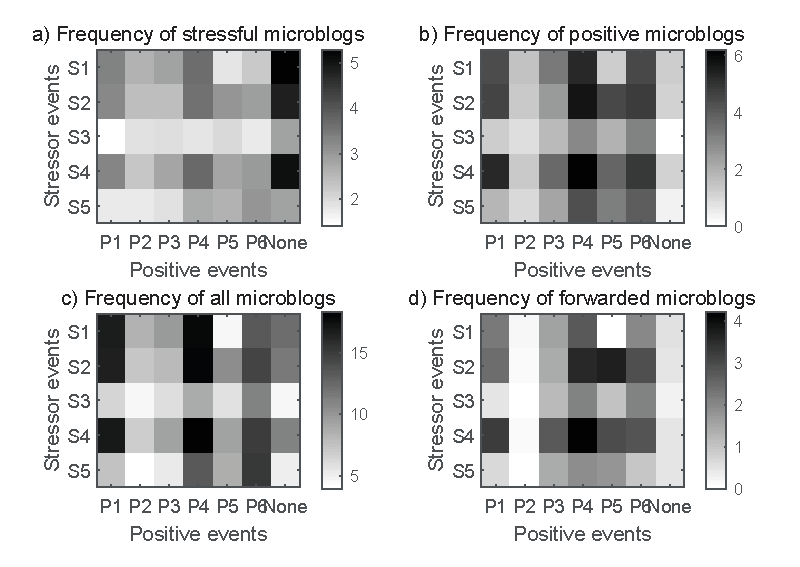
\includegraphics[width=\linewidth]{figs/gray/post.eps}
\caption{\small{Comparing posting behaviors during stressful intervals in SI and U-SI sets.
$P_{1-6}$=\{academic, romantic, peer relationship, self-cognition, family life, entertainment\},
$E_{1-5}$=\{academic, romantic, peer relationship, self-cognition, family life\}.}}
\label{fig:post}
\end{figure}

\paragraph{\textbf{Posting behaviors}}
Stress could lead to abnormal posting behaviors,
reflecting user's changes in social engagement activity ~\citep{Liang2015Teenagers}.
We considered four measures of posting behaviors here.
The first measure was frequency of stressful microblogs,
highlighting stressful microblogs among all microblogs.
Research in \cite{Li2017Analyzing} indicated that overwhelmed adolescents
tended to post more microblogs expressing their stress for releasing and seeking comfort from friends.
The second measure was frequency of positive microblogs,
indicating the number of positive microblogs per day.
The third measure was the total number of all microblogs per day.
The forth measure was frequency of forwarded microblogs,
showing the number of re-tweet and shared microblogs.
Figure \ref{fig:post} summarized the distribution of above four measures in U-SI and SI sets.
Results in subgraph (a) and (b) showed decrease of stressful microblogs and
increase of positive microblogs when positive events occurred.
Subgraph (d) indicated adolescents tended to forward more microblogs when positive events happened,
while subgraph (c) showed that the frequency of all microblogs didn't appear obvious change under the impact of positive events.

\begin{table*}
\begin{center}
\caption{\small{Monotonous stress intensity changes in U-SI and SI intervals compared with adjacent intervals.
 \emph{Front$ \rightarrow$ I} represented monotonous increase from the front interval to current stressful interval $I$.
\emph{I $\rightarrow$ rear} represented monotonous decrease from interval $I$ to its rear interval.
}}
%\resizebox{\textwidth}{15mm}{
\small{
\begin{tabular}{l cccccc cccccc} \\\hline
\multirow{2}{1cm}{}
&\multicolumn{2}{c}{school life}
&\multicolumn{2}{c}{romantic}
&\multicolumn{2}{c}{peer relationship}
&\multicolumn{2}{c}{self-cognition}
&\multicolumn{2}{c}{family life}
&\multicolumn{2}{c}{all types}\\
&U-SI	    &	SI	        &U-SI	    &SI	        &U-SI	   &SI	
&U-SI	    &	SI	        &	U-SI	&SI	        &U-SI	   &SI\\  \hline
\# interval         &   365	        &	514	        &	536	        &	587	        &128	    &	391	        &	564	           &	609	            &	321	        &	481	        &	1,914	    &2,582	 \\
front $\rightarrow$ I &	72.60\% &	78.79\% &	69.03\% 	&77.51\%   &74.22\%    &81.59\%    &70.04\%    &77.67\%  &67.91\%     &77.96\%    &70.17\%    &78.51\% \\
I $\rightarrow$ rear  &	75.89\% &	78.40\% &	74.63\% 	&79.05\%   &78.13\%    &82.61\%    &75.00\%    &79.15\%   &74.14\%    &79.42\%    &75.13\%    & 79.55\%\\ \hline
\end{tabular}}%}}
\label{tab:fontrear}
\end{center}
\end{table*}

\subsubsection{Monotonous Model of Stress-buffering}
\label{sec:mono}
To further verify the monotonous changes of stress intensity under the impact of positive events,
for each stressful interval in SI (n=2,582) and U-SI (n=1,914) sets,
we compared its stress intensity with the front and rear adjacent intervals respectively.
For a stressful interval $I = <t_i,t_{i+1},\cdots,t_j>$,
let $I^{front} = <t_m,\cdots,t_{i-1}>$ be the adjacent interval before $I$,
and $I^{rear} = <t_{j+1},\cdots,t_n>$ be the rear adjacent interval of $I$.
The length of $I^{front}$ and $I^{rear}$ were set to $|I|$.
For the set of stressful intervals $SI$ composed of $<I_1,I_2,\cdots,I_N>$,
the corresponding sets of adjacent front and rear intervals were denoted as $SI^{front}$ and $SI^{rear}$.
Similarly, for the set of stressful intervals $USI$ = $<UI_1,UI_2,\cdots, UI_M>$ impacted by positive events,
the corresponding sets of adjacent front intervals and adjacent rear intervals were denoted as $USI^{front}$ and $USI^{rear}$.
We compared the intensity of stress changes in following four situations,
where $g(.)$ was the function comparing two sets: \\
1) $g(SI,SI^{front}$) returned if intensive change happened when stressful intervals begin.\\
2) $g(SI,SI^{rear}$) returned if stress changes intensively after the stressful intervals end.\\
3) $g(USI,USI^{front}$) returns if intensive change happened when stressful intervals affected by positive events.\\
4) $g(USI,USI^{rear}$) returns if stress changed intensively after stressful intervals affected by positive events.

In our problem, taking the comparison between $SI$ and $SI^{rear}$ for example,
the basic computation element $I_k \in SI \cup SI^{rear}$ in both sets was an interval, denoted as a multi-dimension point.
Here we adopt the t-test method as the intensity computation function $g(.)$.
The function $g(.) = t_{score}$ $\in$ (-1,1) was represented as:

\begin{equation}
\small{g(SI,SI^{rear})}= \frac{\mu_{SI}-\mu_{SI^{rear}}}{\sqrt{\frac{(n_1-1)\sigma^2_{SI}+(n_2-1)\sigma^2_{SI^{rear}}}{n_1+n_2-2}(\frac{1}{n_1}-\frac{1}{n_2})}}
\end{equation}
where $\mu_{SI}$ and $\mu_{SI^{rear}}$ were the mean stress values of intervals in sets $SI$ and $SI^{rear}$,
and $\sigma_{SI}$ and $\sigma_{SI^{rear}}$ were the variance stress values of intervals in sets $SI$ and $SI^{rear}$, respectively.
If $g(SI,SI^{rear})$ $> \alpha$, stress intensity in $SI^{rear}$ showed significant decrease compared with $SI$ (monotonic negative effect).
If $g(SI^{front},SI)$ $< -\alpha$, stress intensity in $SI$ showed significant increase compared with $SI^{front}$ (monotonic positive effect).
Here we adopted $\alpha$ = 1.96, $P$ = 0.025.
We conducted comparison for above four situations
to observe whether the occurrence of positive events relieved the monotonic negative effect of $g(SI,SI^{rear})$
and the monotonic positive effect of $g(SI^{front},SI)$.

\section{Experiments}
\subsection{Stress-buffering Effect of Positive Events}
\label{subsec:experiment}
\begin{table}[h]
\begin{center}
\caption{\small{Quantify the stress-buffering effect of scheduled positive events applying KTS model (the KNN-based two sample method adopted in this research) and baseline method.}}
\label{tab:schedule}
\resizebox{0.45\textwidth}{13mm}{
\small{
\begin{tabular}{lccccc}
\toprule
&	practical	&	         	&	new year	&	sports	&	\\
&	activity	&	holiday	&	party	&	meeting	&	all	\\
\midrule
size of U-SI	&	219 	&	339 	&	235 	&	226 	&	1,019 	\\
Pearson         &55.65\%	&	70.97\%	&	56.45\%	&	54.84\%	&	65.32\% \\
KTS             &54.52\%	&	78.39\%	&	63.39\%	&	58.74\%	&	69.52\% \\
\bottomrule
\end{tabular}
}
}
\end{center}
\end{table}
Basically, we explored the stress-buffering effect of specific positive events based on the framework in section \ref{sec:frame}.
Four scheduled positive events were adopted:
practical activity, holiday, new year party and sports meeting.
Table \ref{tab:schedule} showed the experimental results,
where 54.52\%, 78.39\%, 63.39\%, 58.74\% significant stress-buffering effect were detected for
each of the four scheduled positive events, with the total ratio to 69.52\% ($\alpha$ =1.96 for p=0.025).
Here Pearson correlation algorithm was applied to compare with the statistical model in section \ref{sec:frame2}.
The Euclidean metric was used to calculate the distance between two $n$ dimension points $X$ and $Y$.
Experimental results showed that our KNN-based two sample method (denoted as KTS) outperformed the baseline method
with the best improvement in event \emph{new year party} to 10.94\%, and total improvement to 6.00\%.

\begin{figure}[h]
\centering
\includegraphics[width=\linewidth]{figs/cor.eps}%figs/correlation2.eps
\caption{\small{ Subgraph (a) showed statistical value $\alpha$ of each group of measures.
Subgraph (b) showed stress-buffering effects on five dimensions of stress.}}
\label{fig:correlation}
\end{figure}

Stress-buffering effects measured by three groups of microblog characteristics and towards five dimensions of stressor events were shown in box-plots \ref{fig:correlation},
using the statistical value $\alpha$ computed through KTS method.
Results showed the stress-buffering pattern of positive events
was significantly correlated with posting behaviors (ratio = 83.06\%, n=103, SD=1.96),
stress change modes (ratio = 74.19\%, n=92, SD=2.04) and linguistic expressions (ratio = 77.42\%, n=96, SD=2.07).
Positive events conducted most significant stress-buffering impact on 'family life' (ratio = 84.68\%, n=105, SD=2.72),
followed by 'peer relationships' (ratio = 79.03\%, n=98, SD=4.04) and 'academic' (ratio = 68.55\%, n=85, SD=2.71) dimensions.
Statistics $\alpha$ in 'peer relation'
exhibited the highest 75th percentile while the lowest 25th percentile,
showing a relatively random and unstable stress-buffering effect on this dimension.
Comparing the hypothesis test results on scheduled positive events (ratio = 69.52\%)
and automatically extracted positive events (ratio = 74.21\%),
the result indicated the feasibility of automatically extracting positive events from microblogs.

Next,
to verify monotonous changes of stress intensity when an positive event impacted a stressful interval,
for each interval in SI and U-SI sets,
we quantified its monotonous stress changes by comparing with the front and rear adjacent intervals, respectively.
Four situations proposed in section \ref{sec:mono} were considered and compared in table \ref{tab:fontrear}.
The ratio of intervals detected with monotonous increase from the front interval to current stressful interval $I$ (denoted as \emph{front$ \rightarrow$ I}),
and ratio of monotonous decrease from $I$ to its rear interval (denoted as \emph{I $\rightarrow$ rear}) were summarized.
Under the effect of positive events,
the ratio of intensive stress increase in \emph{front$ \rightarrow$ I} was decreased from 78.51\% to 70.17\%;
and the ratio of intensive stress decrease in \emph{I $\rightarrow$ rear} was decreased from 79.55\% to 75.13\%.
The most obvious monotonous decrease in \emph{front$ \rightarrow$ I} was conducted by positive events in family life dimension (12.89\% reduction);
and the most obvious monotonous decrease in \emph{front$ \rightarrow$ I} was also conducted by positive events in family life dimension (6.65\% reduction).
The experimental results indicated the effectiveness of the two sample method for quantifying the effect of positive events,
and the rationality of the assumption that positive events could help ease stress of overwhelmed adolescents.


\begin{table*}
\caption{Adolescents' stress prediction performance when combined different groups of stress-buffering measures separately.}
\begin{minipage}{\linewidth}
\centering
\resizebox{\textwidth}{20mm}{
\begin{tabular}{l cccc cccc cccc cccc} \\\hline%\toprule
\multirow{2}{1cm}{}&\multicolumn{4}{c}{None}
    &\multicolumn{4}{c }{Positive (L)}
    &\multicolumn{4}{c }{Positive (S)}
    &\multicolumn{4}{c}{Positive (P)}\\
    &\scriptsize{MSE} &\scriptsize{RMSE} &\scriptsize{MAPE} &\scriptsize{MAD}
    &\scriptsize{MSE} &\scriptsize{RMSE} &\scriptsize{MAPE} &\scriptsize{MAD}
    &\scriptsize{MSE} &\scriptsize{RMSE} &\scriptsize{MAPE} &\scriptsize{MAD}
    &\scriptsize{MSE} &\scriptsize{RMSE} &\scriptsize{MAPE} &\scriptsize{MAD} \\\midrule					
School life
&   0.0856 	&	0.2926 	&	0.4852 	&	0.1146	&	0.0259 	&	0.1609 	&	0.2991 	&	0.0923 	
&	0.0297 	&	0.1723 	&	0.3135 	&	0.0899 	&	0.0223 	&	0.1493 	&	0.3438 	&	0.0931 	\\
Romantic
&   0.0703 	&	0.2651 	&	0.3555 	&	0.1083 	&	0.0291 	&	0.1706 	&	0.2832 	&	0.0919 	
&	0.0379 	&	0.1947 	&	0.2941 	&	0.1026 	&	0.0332 	&	0.0835 	&	0.2746 	&	0.1240 	\\
Peer relationship
&   0.2800 	&	0.5292 	&	0.3256 	&	0.1697 	&	0.3140 	&	0.5604 	&	0.3626 	&	0.1202 	
&	0.2972 	&	0.5452 	&	0.3060 	&	0.1298 	&	0.2557 	&	0.1472 	&	0.3481 	&	0.1458 	\\
Self-cognition
&   0.0445 	&	0.2110 	&	0.3066 	&	0.1895 	&	0.0345 	&	0.1857 	&	0.2721 	&	0.1653 	
&	0.0366 	&	0.1913 	&	0.2557 	&	0.0754 	&	0.0245 	&	0.0862 	&	0.2863 	&	0.1447 	\\
Family life
&   0.1602 	&	0.4002 	&	0.3291 	&	0.1587 	&	0.0889 	&	0.2982 	&	0.2891 	&	0.0944 	
&	0.0378 	&	0.1944 	&	0.2952 	&	0.0842 	&	0.1827 	&	0.0979 	&	0.3148 	&	0.1131 	\\
All	
&   0.1281 	&	0.3579 	&	0.3604 	&	0.1482	&	0.0985 	&	0.3138 	&	0.3012 	&	0.1128 	
&	0.0878 	&	0.2964 	&	0.2929 	&	0.0964 	&	0.1037 	&	0.1128 	&	0.3135 	&	0.1241 	\\ \hline
\end{tabular}}
\end{minipage}\\
\begin{minipage}{\linewidth}
\centering
\resizebox{\textwidth}{20mm}{
\begin{tabular}{l cccc cccc cccc cccc} \\\hline%\toprule
\multirow{2}{1cm}{}&\multicolumn{4}{c}{Positive (L\&S)}
    &\multicolumn{4}{c }{Positive (L\&P)}
    &\multicolumn{4}{c }{Positive (S\&P)}
    &\multicolumn{4}{c}{Positive (L\&S\&P)}\\
    &\scriptsize{MSE} &\scriptsize{RMSE} &\scriptsize{MAPE} &\scriptsize{MAD}
    &\scriptsize{MSE} &\scriptsize{RMSE} &\scriptsize{MAPE} &\scriptsize{MAD}
    &\scriptsize{MSE} &\scriptsize{RMSE} &\scriptsize{MAPE} &\scriptsize{MAD}
    &\scriptsize{MSE} &\scriptsize{RMSE} &\scriptsize{MAPE} &\scriptsize{MAD} \\\midrule					
School life
&	0.0283 	&	0.1682 	&	0.2934 	&	0.0824 	&	0.0261 	&	0.1616 	&	0.2770 	&	0.0768 	
&	0.0342 	&	0.1849 	&	0.2629 	&	0.0590 	&	0.0132 	&	0.1149 	&	0.2364 	&	0.0717 	\\
Romantic
&	0.0219 	&	0.1480 	&	0.2532 	&	0.0839 	&	0.0180 	&	0.1342 	&	0.2644 	&	0.0952 	
&	0.0176 	&	0.1327 	&	0.2549 	&	0.0823 	&	0.0251 	&	0.1584 	&	0.2507 	&	0.0891 	\\
Peer relationship
&	0.2361 	&	0.4859 	&	0.3182 	&	0.1300 	&	0.2349 	&	0.4847 	&	0.3283 	&	0.1189 	
&	0.2351 	&	0.4849 	&	0.3558 	&	0.1297 	&	0.2341 	&	0.4838 	&	0.3096 	&	0.1093 	\\
Self-cognition
&	0.0329 	&	0.1814 	&	0.2942 	&	0.0946 	&	0.0262 	&	0.1619 	&	0.2791 	&	0.0858 	
&	0.0245 	&	0.1565 	&	0.2740 	&	0.0945 	&	0.0144 	&	0.1200 	&	0.2580 	&	0.0739 	\\
Family life
&	0.1489 	&	0.3859 	&	0.2750 	&	0.1244 	&	0.0395 	&	0.1987 	&	0.2853 	&	0.0939 	
&	0.0484 	&	0.2200 	&	0.2946 	&	0.0992 	&	0.0378 	&	0.1944 	&	0.2645 	&	0.0848 	\\
All
&	0.0936 	&	0.3060 	&	0.2868 	&	0.1031 	&	0.0689 	&	0.2626 	&	0.2868 	&	0.0941 	&	0.0720 	&	0.2683 	&	0.2884 	&	0.0929 	&	0.0649 	&	0.2548 	&	0.2638 	&	0.0858 	\\ \hline
\end{tabular}}
\begin{tablenotes}
        \footnotesize
        \item[1] $^1$ Three stress-buffering measures: 'L' represents \emph{linguistic expression}, 'S' represents \emph{stress intensity}, and 'P' represents \emph{posting behavior}.
      \end{tablenotes}
\end{minipage}
\label{tab:forecast}
\end{table*}

\subsection{Predicting Future Stress Under the Stress-buffering Effects of Positive Events}
\label{subsec:predict}
To further explore the effectiveness of our method for quantifying stress-buffering effects of positive events,
we integrate the impact of positive events into a stress prediction problem,
and verify whether considering stress-buffering effects of positive events could help improve stress prediction performance.


\paragraph{Stress prediction model}
The SVARIMA (Seasonal Autoregressive Integrated Moving Average) algorithm was proved to be suitable for adolescents' stress prediction problem \citep{Li2015Predicting, Shumway2006Time},
due to the seasonality and non-stationarity of stress series.
Since stressor events cause the fluctuation of stress series from normal states,
we focused the prediction problem on stressful intervals rather than randomly picked out stress series.
Thus the basic stress prediction was conducted using SVARIMA approach in the set of stressful intervals impacted by positive events (U-SI).
Stress-buffering effects of positive events were adopted as adjust values to modify stress prediction results.
Four metrics were adopted to measure stress forecasting performance,
where \emph{MSE}, \emph{RMSE} and \emph{MAD} measured absolute errors and \emph{MAPE} measures relative errors.
For all real stress value $\overline{s_i}$ and predicted stress value $s_i$ in predicting sequence $<s_1,\cdots,s_n>$:
$MSE = \frac{1}{n}\sum_{i\in[1,n]}(s_i-\overline{s_i})^2$,
$RMSE = \frac{1}{n}\sqrt{\sum_{i\in[1,n]}(s_i-\overline{s_i})^2}$,
$MAD = \frac{1}{n}\sum_{i\in[1,n]}|s_i-\overline{s_i}|$,
$MAPE = $ $\frac{1}{n}$ $\sum_{i\in[1,n]}{|s_i-\overline{s_i}|/s_i}$.

The experimental set contained 1,914 stressful intervals under the impact of positive events (U-SI).
As shown in Table \ref{tab:forecast},
the original prediction performance using only SVARIMA method
achieved 0.1281 MSE, 0.3579 RMSE, 0.3604 MAPE and 0.1482 MAD ($L = 7$, $\beta = 0.5$).
Then we integrated the stress-buffering impact of each dimension of positive events into stress prediction.
Specifically, for positive events conducted significant stress-buffering effects on current adolescent,
the average stress value during historical U-SI intervals were integrated to modify the result by adjusting the parameter $\beta$.
After modification,
the prediction performance achieved 0.0649 MSE,	0.2548 RMSE, 0.2638 MAPE and 0.0858 MAD,
reducing the prediction errors efficiently (with MSE, RMSE, MAPE and MAD reduced by 49.34\%, 28.81\%, 26.80\% and 42.11\%, respectively).

\paragraph{Contribution of each group of measures}
Further,
we conducted experiments with different stress-buffering patterns included respectively,
thus to show its contribution to stress prediction.
Four groups of situations were considered here, as shown in Table \ref{tab:forecast},
considering
1) all three groups of measures, namely stress change modes, linguistic expressions and post behaviors (the L\&S\&P pattern),
2) any two of the three groups of measures included (the L$|$S, L\&P, and S\&P patterns),
3) only one group of measures included (the L, S, or P patterns),
and 4) none group of measures included.
We integrated the effect of positive events under the four situations into stress prediction by overlapping paramiter $\alpha \times S_{historical}$,
where $S_{historical}$ was average stress value in historical U-SI intervals.
Here we present the prediction result when $\beta = 0.5$ in each dimension of stress respectively.
Results showed that stress-buffering pattern in L\&S\&P pattern outperformed other patterns
(0.0649 MSE, 0.2548 RMSE, 0.2638 MAPE and 0.0858 MAD),
showing the effectiveness of all three groups of measures.
\begin{figure*}
\centering
\caption{Adolescents' stress prediction performance under different lengths of observation windows.}
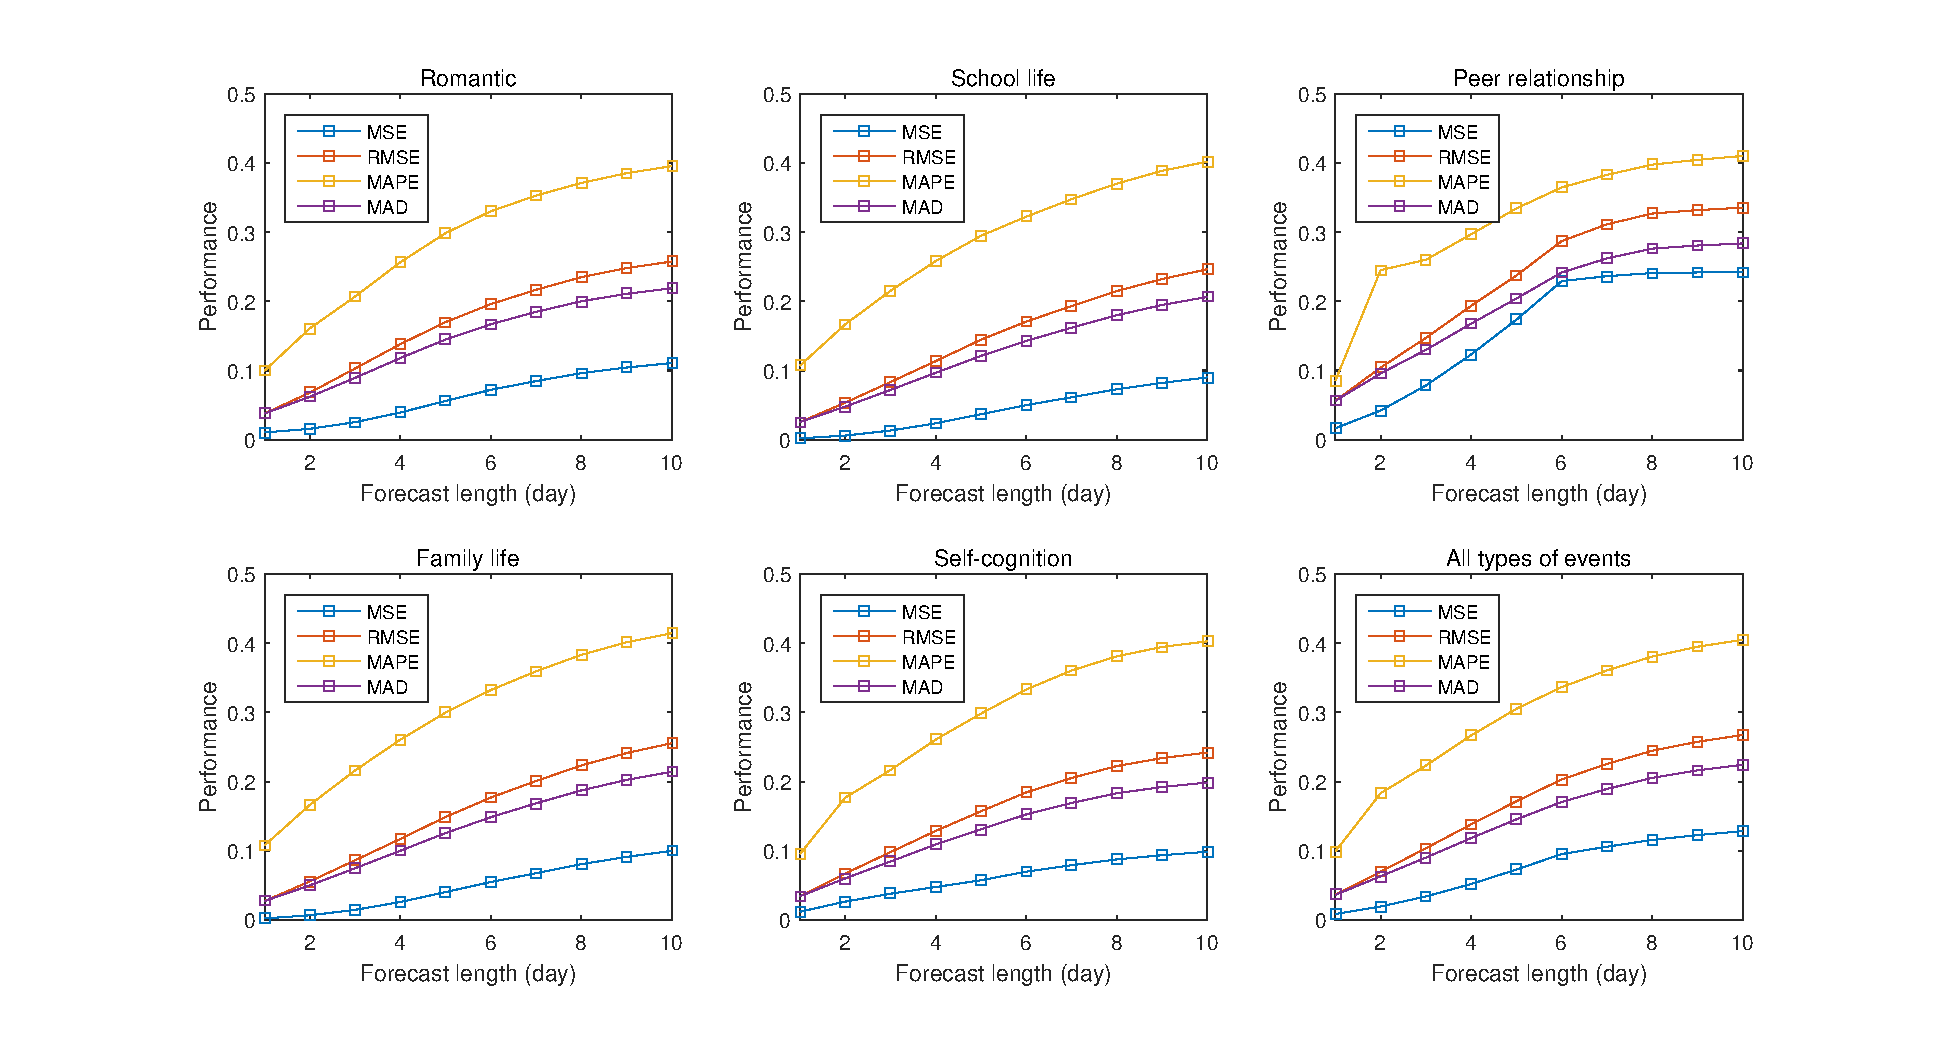
\includegraphics[width=\linewidth]{figs/predictWindow2.eps}
\label{fig:length}
\end{figure*}

\paragraph{Stress prediction performance under different observation windows}
We further explored to combine stress-buffering effects into future stress prediction under different length of observation windows, ranging from 1 to 10 days, as shown in Figure \ref{fig:length}.
With window length increasing,
prediction errors showed increasing trend in all metrics.
The reason might be that longer prediction window took more previous predicted results,
and errors accumulates with more predicted values taken into the next step prediction.
Among five dimensions of stressor events,
prediction for school life stress achieved the best performance.
One reason might be more positive events and stressors about school life events were detected from adolescents' microblogs,
providing sufficient data in prediction process.
On the other side,
stress coming from school life was the most common stress in student group,
with relative stable periodicity,
which was more suitable for current prediction model.


\begin{figure}
\centering
\caption{Stress prediction performance under L\&S\&P stress-buffering pattern of positive events.}
\includegraphics[width=\linewidth]{figs/thresh.eps}
\label{fig:thresh}
\end{figure}

\paragraph{Parameter settings}
Parameter $\beta$ was adjusted when integrated impact of positive events into stress prediction.
For each of the four groups of stress-buffering patterns,
we adjust $\beta$ in the effect of $\beta \times L$.
We calculated the corresponding prediction result for each adolescent respectively,
and showed the result of whole testing group in average performance.
Figure \ref{fig:thresh} showed the changing trend under the L\&S\&P pattern.
Prediction errors decreased first and then increased,
and the best performance was achieved when $\beta$ was nearby 0.52,
with 0.0649 MSE, 0.2548 RMSE, 0.2638 MAPE and 0.0858 MAD as the average performance of the whole experimental data set.
Multiple methods for integrating stress-buffering impact of positive event into stress prediction could be adopted in the future.
In this paper we adopted the simple one to verify the effectiveness of our model in quantifying the impact of positive events.
The setting of parameter $\beta$ could be changed due to different individuals and data sets.


\section{Discussion}
\label{sec:conclude}
The main contribution of the present study lies in the following three aspects.
First, we validated and expanded the theoretical results of previous studies.
The characteristics of stress-buffering were not only manifested in self-reported subjective feelings,
but also in behavioral level in social networks.
We examined the potential relationship between the occurrence of positive events and the posting behaviors,
microblog contents and stress change mode on stressed adolescents,
and verified that
positive events buffered monotonous stress changes at both the early and late stages.
Second, this study implemented the innovation of methods.
Through building a complete technical framework,
we realized
1) automatic extraction of positive events, as well as users' behavior and content measures from microblogs,
and 2) quantification of relationships between stress-buffering of positive events and microblogging measures.
Third, this article showed practical significance.
It realized timely and continuous monitoring of the stress-buffering process
of adolescents based on public social network data sources,
which could be used to assess the stress resistance of adolescents;
on the other hand, it could provide supplementary advice to schools and parents about
'when to arrange positive events to ease stress of adolescents'.

There were three groups of results in this work.
In study 1, the scheduled school events with exact time intervals and the microblogs posted by a group of 500 students were collected and statistically analyzed.
Results showed that when positive events were scheduled neighboring stressful events,
students exhibited less stress intensity and shorter stressful time intervals from their microblogs.
The study also found that most students talked less about the upcoming or just-finished exams when positive events happened nearby,
with lower frequency and lower ratio.
The results substantiated previous studies reporting the protective effect of positive events on adolescents~\citep{Cohen2010Positive,Shahar2002Positive} using laboratory methods.
Based on this, this article carried out more in-depth follow-up studies.

The second groups of results were presented in study 2,
examining stress-buffering pattern of positive events through microblog content and behavioral measures.
As basis, a complete solution was provided for automatically detecting positive events based on microblog semantics,
which were totally different from traditional questionnaire methods,
enabling timely, fraud-proof and continuous detection.
In order to eliminate the possible errors in positive event detection and avoid false overlays,
we first used four scheduled positive events to examine significant stress-buffering effects.
Results showed the event 'holiday' exhibited the highest proportion of significant stress-buffering.
However, this conclusion was questionable because the frequency of the above four events was different and might affect the experimental results.
Next, the stress-buffering effect of automatically extracted positive events were tested based on three groups of stress-buffering measures.
The most intensive stress-buffering effects were shown in 'school life' and 'peer relationship' dimensions.
\emph{Posting behaviors} exhibited most significant correlations among three groups of measures.
This resonated with the study \cite{BLACHNIO2016664,Disclosure} suggesting that users who
tended to share important news on Facebook had a higher level of stress.

This article proposed a novel perspective to better understand the process of stress-buffering.
Since more complex situations were simplified in the present exploration,
the goals were still salient for stress-buffering researches from social networks.

\section{Limitations and future work}

This study has a number of limitations.
First, it used the microblog data set collected from social networks of high school students,
and chose the scheduled school events as the ground truth in the pilot study.
This could be seen as a relative fuzzy verification method,
because individual events (i.e., 'lost love', or 'received a birthday present') might also conduct additional impact.
Therefore, the data observation in the pilot study were not 100\% rigorous and needed further verification.
A improvement might be conducted by inviting participants to complete related scales (e.g., positive and stressor scales),
thus to label part of the data set,
and achieve a balance between data volume and accuracy.

Second,
this study treated positive events as independent existence and studied the effect of each event separately.
This ignored the additive and collective effects of multiple positive events which might happened at the same time.
Thus, our future research might investigate the overlap effects of multiple positive events,
as well as the frequent co-appearing patterns of different types of positive events,
thus to provide more accurate stress-buffering guidance for individual adolescents.

Based on current research implications,
more factors could help analyze stress-buffering patterns among adolescents more comprehensively in future research.
One factor is how personality ~\citep{personality1,personality2} impacts the stress-buffing effect of positive events,
which could be captured from the social media contents.
Another key factor is the role the social support~\citep{socialSupport1, socialSupport2} in social networks plays.
This factor leaves clues in the messages under each post,
and the behaviors (i.e., retweet, the like numbers) of friends.
For examples, ~\citep{socialSupport1} showed that the number of Facebook friends was associated with stronger perceptions of social support,
which in turn correlated with reduced stress and greater well-being.
The corresponding experimental design, and the online-offline complementary verification will be challenges in the future work.


\section{Reference}
\bibliographystyle{model4-names}
\bibliography{reference-new}
\end{document}
